\section{Other Approaches}
\label{appendix:other}

In this section we briefly describe some other methods that we tried but which either failed or did not produce the desired results.

\subsection{Naive approach}
Initially we attempted to pass the RGB frames directly to the neural network (CNN followed by fully-connected layers). 
The intent was provided to the fully-connected layers as a one-hot encoded vector. We observed that the model drove forward, but generalized poorly and had issues remaining within the lanes. 
We hypothesize that the approach likely failed because the model used complete frames as input. It was therefore required to learn both relevant input features and the control policy simultaneously, which is a difficult task when data is limited.
Additionally, we believe that the conditioning method was too weak to give the model a sufficient learning signal.

\subsection{Classification}
\label{subsec:class_strat}
As described in section \ref{sec:datacollection}, we utilized discrete control signals during the data collection phase. Inspired by this, we attempted to train the model to accurately predict appropriate actions given the current input frame. 
The output layer therefore consisted of 3 neurons, referring to the actions: W = "straight", W + A = "left turn" and W + D = "right turn". We tried this in combination with the multiple head architecture from Section \ref{subsec:mh} and 
observed that the model was able to control the Duckiebot, but also demonstrated a highly non-smooth and zigzagy driving style. For this reason we decided not to pursue the approach any further.

\subsection{Time-Shift Regularization}
\label{appendix:regularization}


Beyond the architectural and task-based approaches, we experimented with regularization techniques. During deployment, we observed a consistent sensitivity to intent changes, suggesting the learned policies were overfitting to the expert policy in the training data. To address this, we implemented time-shift regularization, which involves shifting intent and velocity labels by a small number of time steps relative to the ground truth. This approach assumes that the expert policy is stochastic; therefore, intents or velocities remain valid across a range of time steps. We also hypothesized that this would increase robustness to latency errors, which accumulate when the model is deployed on a remote machine rather than locally on the Duckiebot.

To test this, we trained the FiLM architecture with various time-shift values and qualitatively evaluated its performance on the Duckiebot. The regularization was implemented as a Gaussian distribution around the ground truth timestamp (illustrated in Figure \ref{fig:time_shift_distributions}). Given the 10Hz data collection rate, we tested velocity and intent label shifts at a standard deviation of 0.1s, both independently and in combination. Additionally, we tested a combined shift using a standard deviation of 0.05s, both with and without a 0.05s mean shift into the future.

\begin{figure}[H]
    \centering
    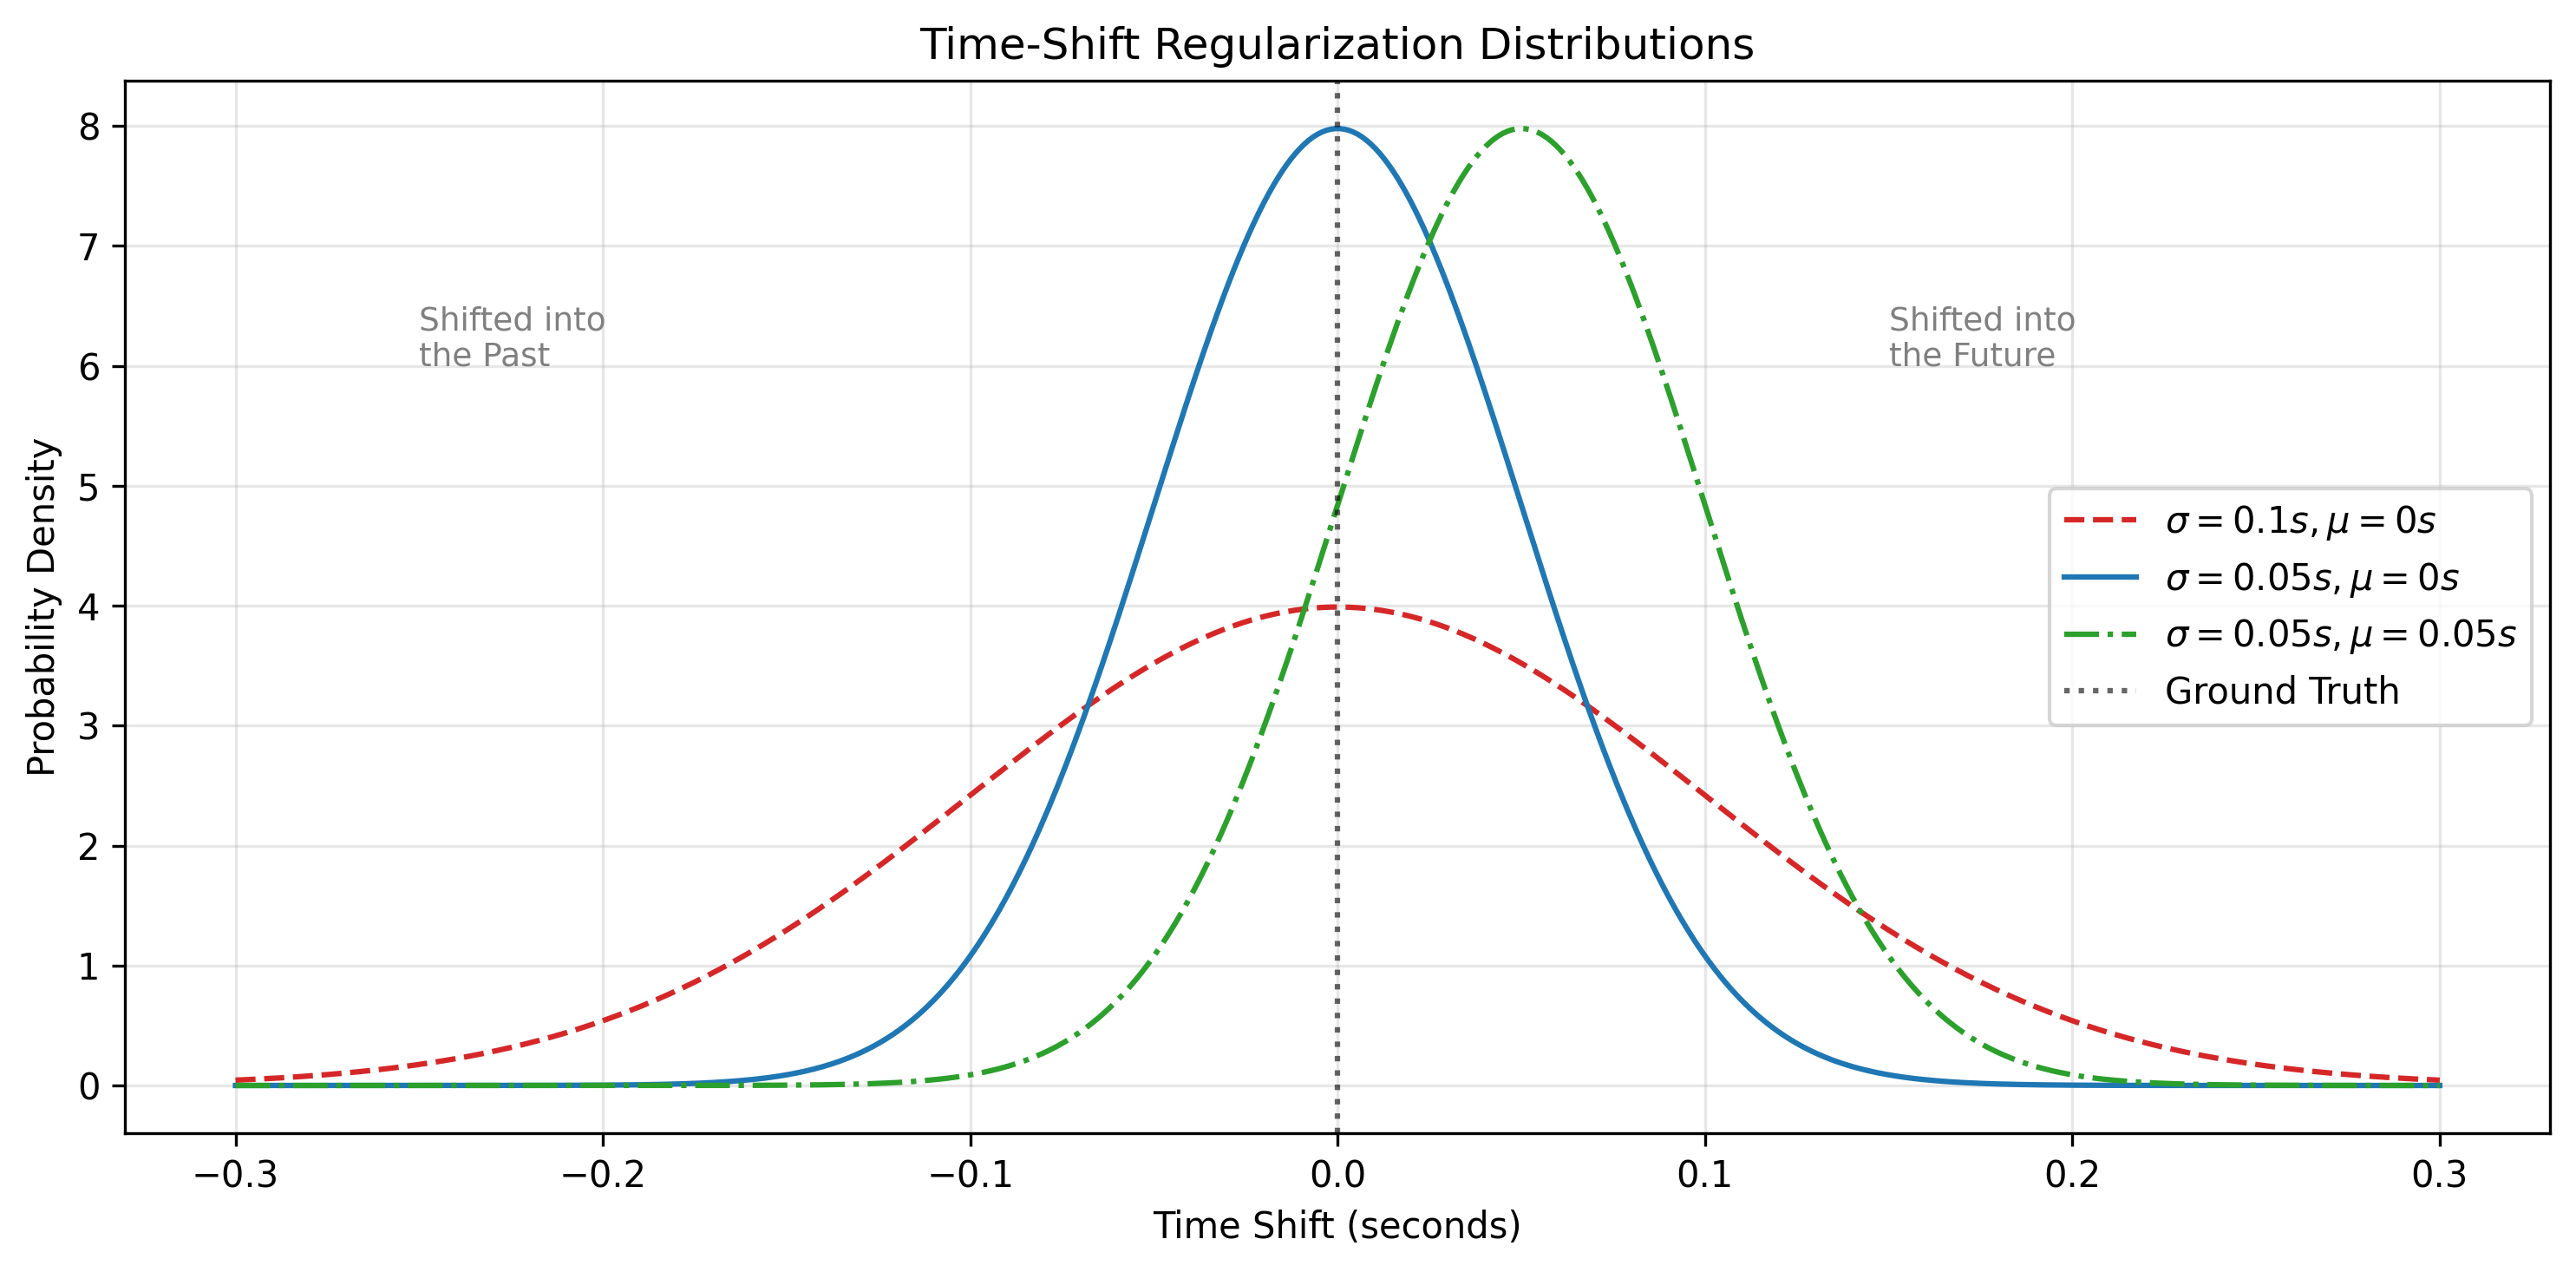
\includegraphics[width=0.8\textwidth]{images/ablation/regularization/time_shift_distributions.png}
    \caption{\textbf{Time-shift regularization:} The figure illustrates the Gaussian distributions used for time-shift regularization.}
    \label{fig:time_shift_distributions}
\end{figure}

Results indicated that these models generally underperformed compared to the baseline. Specifically, the Duckiebot frequently failed to maintain its lane and showed no significant improvement in intersection maneuvers. While the models improved at maintaining a straight path at intersections, they still trailed the baseline model trained with the sampling strategy described in Section \ref{sec:results}. Among the variants, the model with a 0.05s standard deviation and mean shift performed best, whereas all models with a 0.1s standard deviation performed worst. We suspect that shifting labels into the past causes the model to learn a policy that lacks the reactivity required for lane following. Shifting the Gaussian mean into the future reduced the likelihood of past-label shifts, likely accounting for that model’s superior performance. Given these results, we chose to prioritize other approaches rather than further investigate these temporal shifts.

\subsection{Sim2Real Transfer}
\label{appendix:rsim2real}

Like the vast majority of deep learning applications, conditional imitation learning is exceedingly data hungry. Further more, the continuous, stochastic and partially-observable characteristics 
of the environment the duckiebot needs to navigate exacerbates the issue. Even with a strong assumption/bias regarding the duckietown layout, approximately 11,000 samples were required for the CIL 
models to reach the performance documented in this report. If the findings here are eventually expanded further into novel or more complex environments, a question that naturally arises is how to collect 
the vast amounts of required data in a scalable fashion. We set out to evaluate the suitability of the simulation engine Duckiematrix for this purpose.

Since our pipeline follows a two-stage approach where the scene is first summarized into a semantic mask and a policy network subsequently predicts wheel velocities, our ablation study also focuses 
on each component separately. Firstly, two datasets were collected using the same expert policy, with one being collected within the Duckiematrix environment and the other in real life on the physical duckiebot. 
Both datasets were subsequently balanced to contain roughly the same distribution over intent classes, meaning that intersection and lane scenarios were represented equally in each. The first ablation 
involved investigating the sim2real transfer of the YOLO model in terms of semantic segmentation performance. For this, the SAM 3 foundation model was used to annotate both the virtually and physically collected data 
and YOLO26n semantic segmentation models were fine-tuned utilizing the resulting masks of lane markings. In the end, three YOLO26n variants were trained; one on only virtual Duckiematrix data, one on 
solely physical data and one model after merging both data sources. All YOLO26n models were then evaluated quantitatively and qualitatively on the physically collected data, as this is the modality one ultimately wants to predict. 
Samples are shown in Figure \ref{fig:sample_masks}. All models generally segmented accurately in regions close to the camera, but especially the model trained only on virtual data struggled to classify predictions correctly.

\begin{figure}[H]
    \centering
    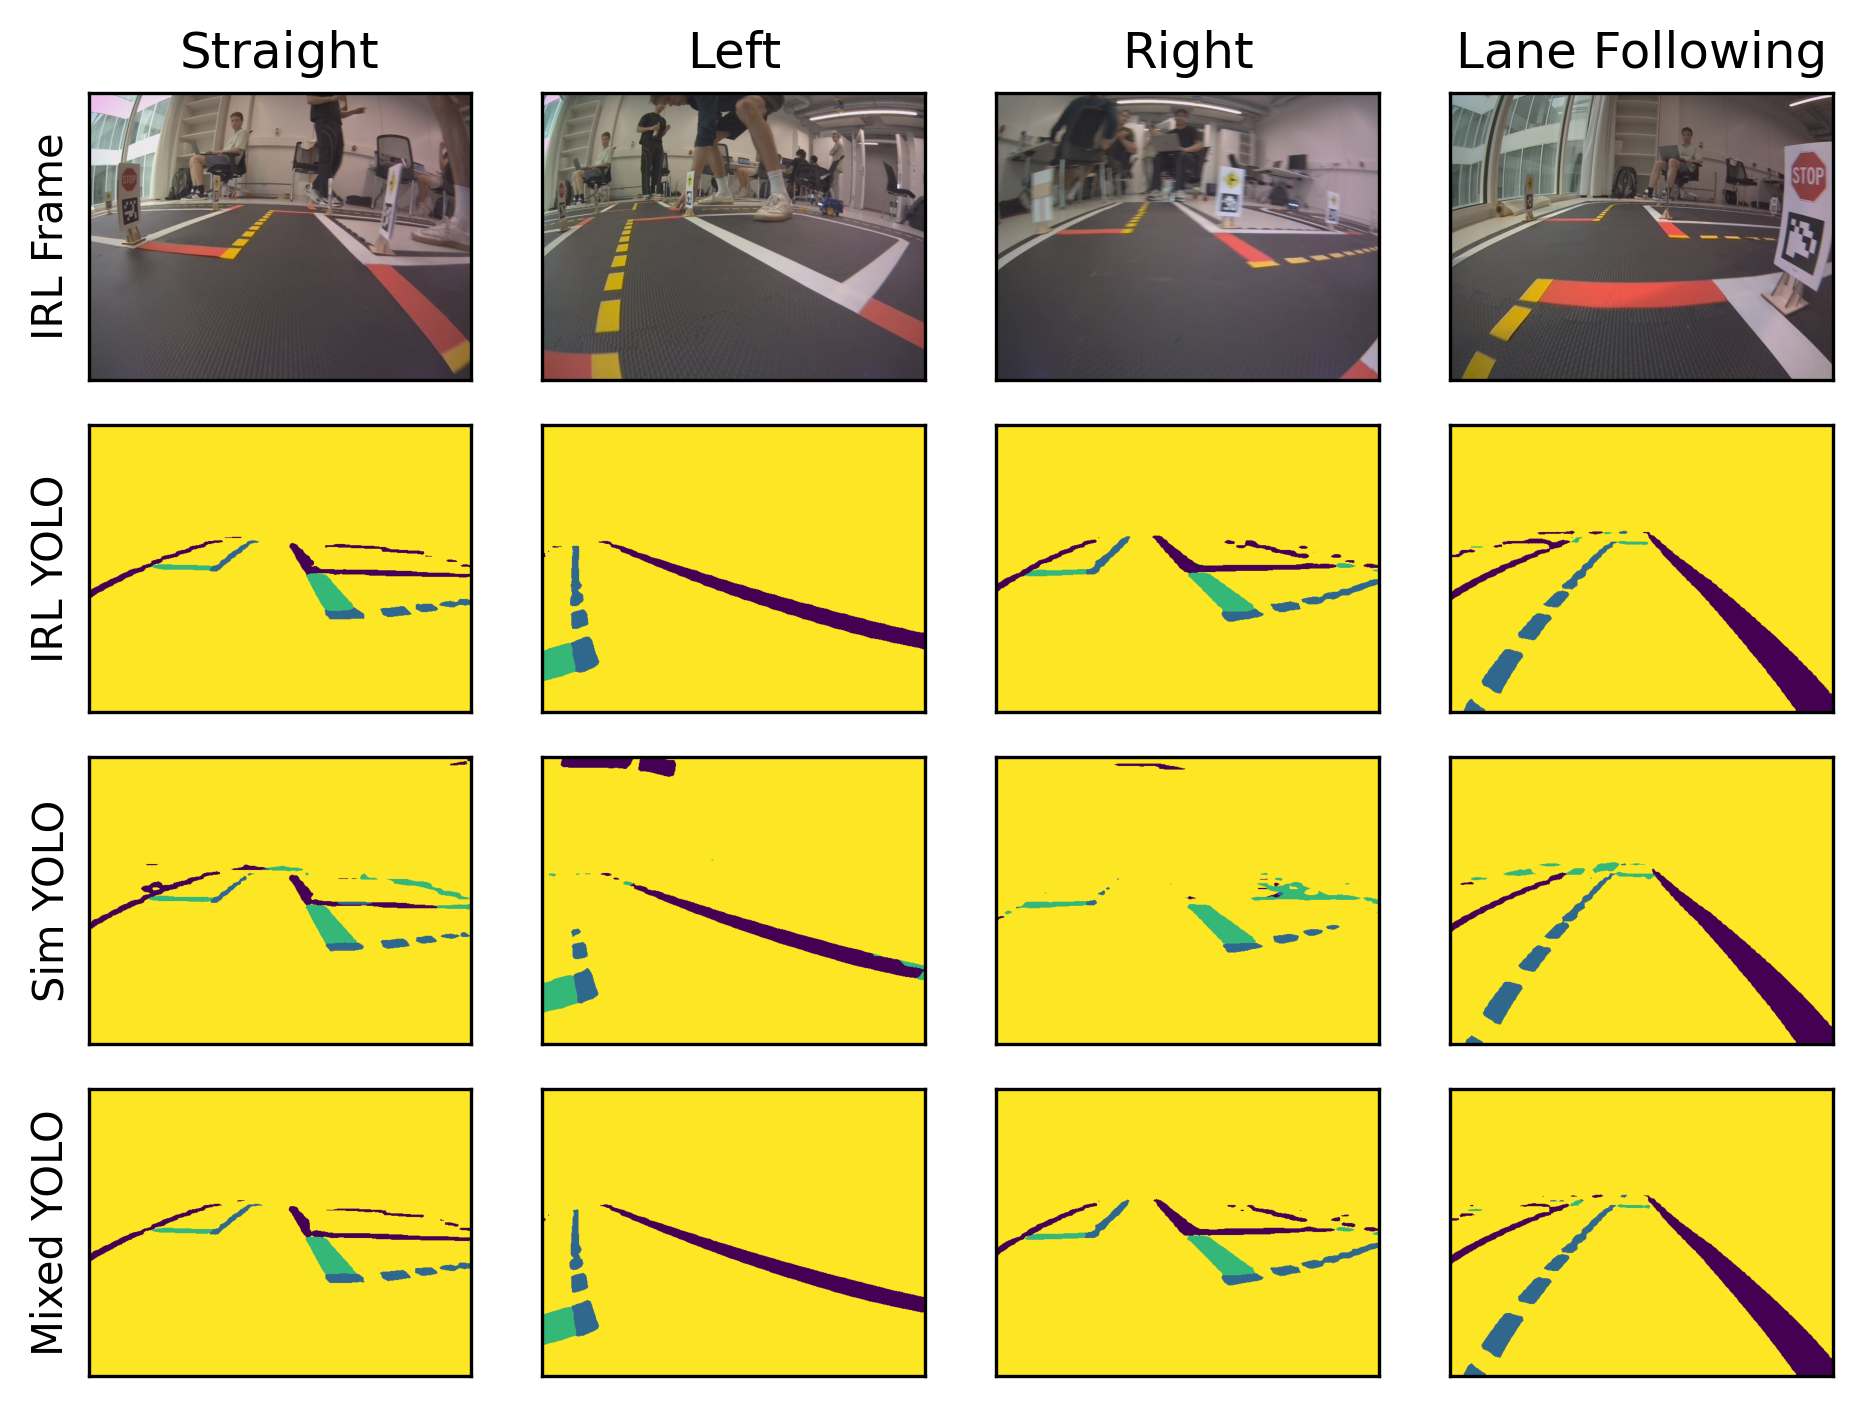
\includegraphics[width=0.8\textwidth]{images/ablation/segmentation/sample_masks_all.png}
    \caption{\textbf{Segmentation Samples:} The figure shows samples from each YOLO26n model trained on either virtual, physical or all data.}
    \label{fig:sample_masks}
\end{figure}

The second ablation we did was regarding the policy network. For all experiments we used the multi-head model depicted in Figure \ref{fig:multipleHeads}. We again trained three variants using virtual data, physical data or both and 
utilized the corresponding YOLO26n model, trained in the first ablation, for each. Subsequently we evaluated their ability to predict the wheel velocities of the physical data. Results are shown in Figure \ref{fig:perf_transfer}

\begin{figure}[H]
    \centering
    \begin{subfigure}[b]{0.8\textwidth}
        \centering
        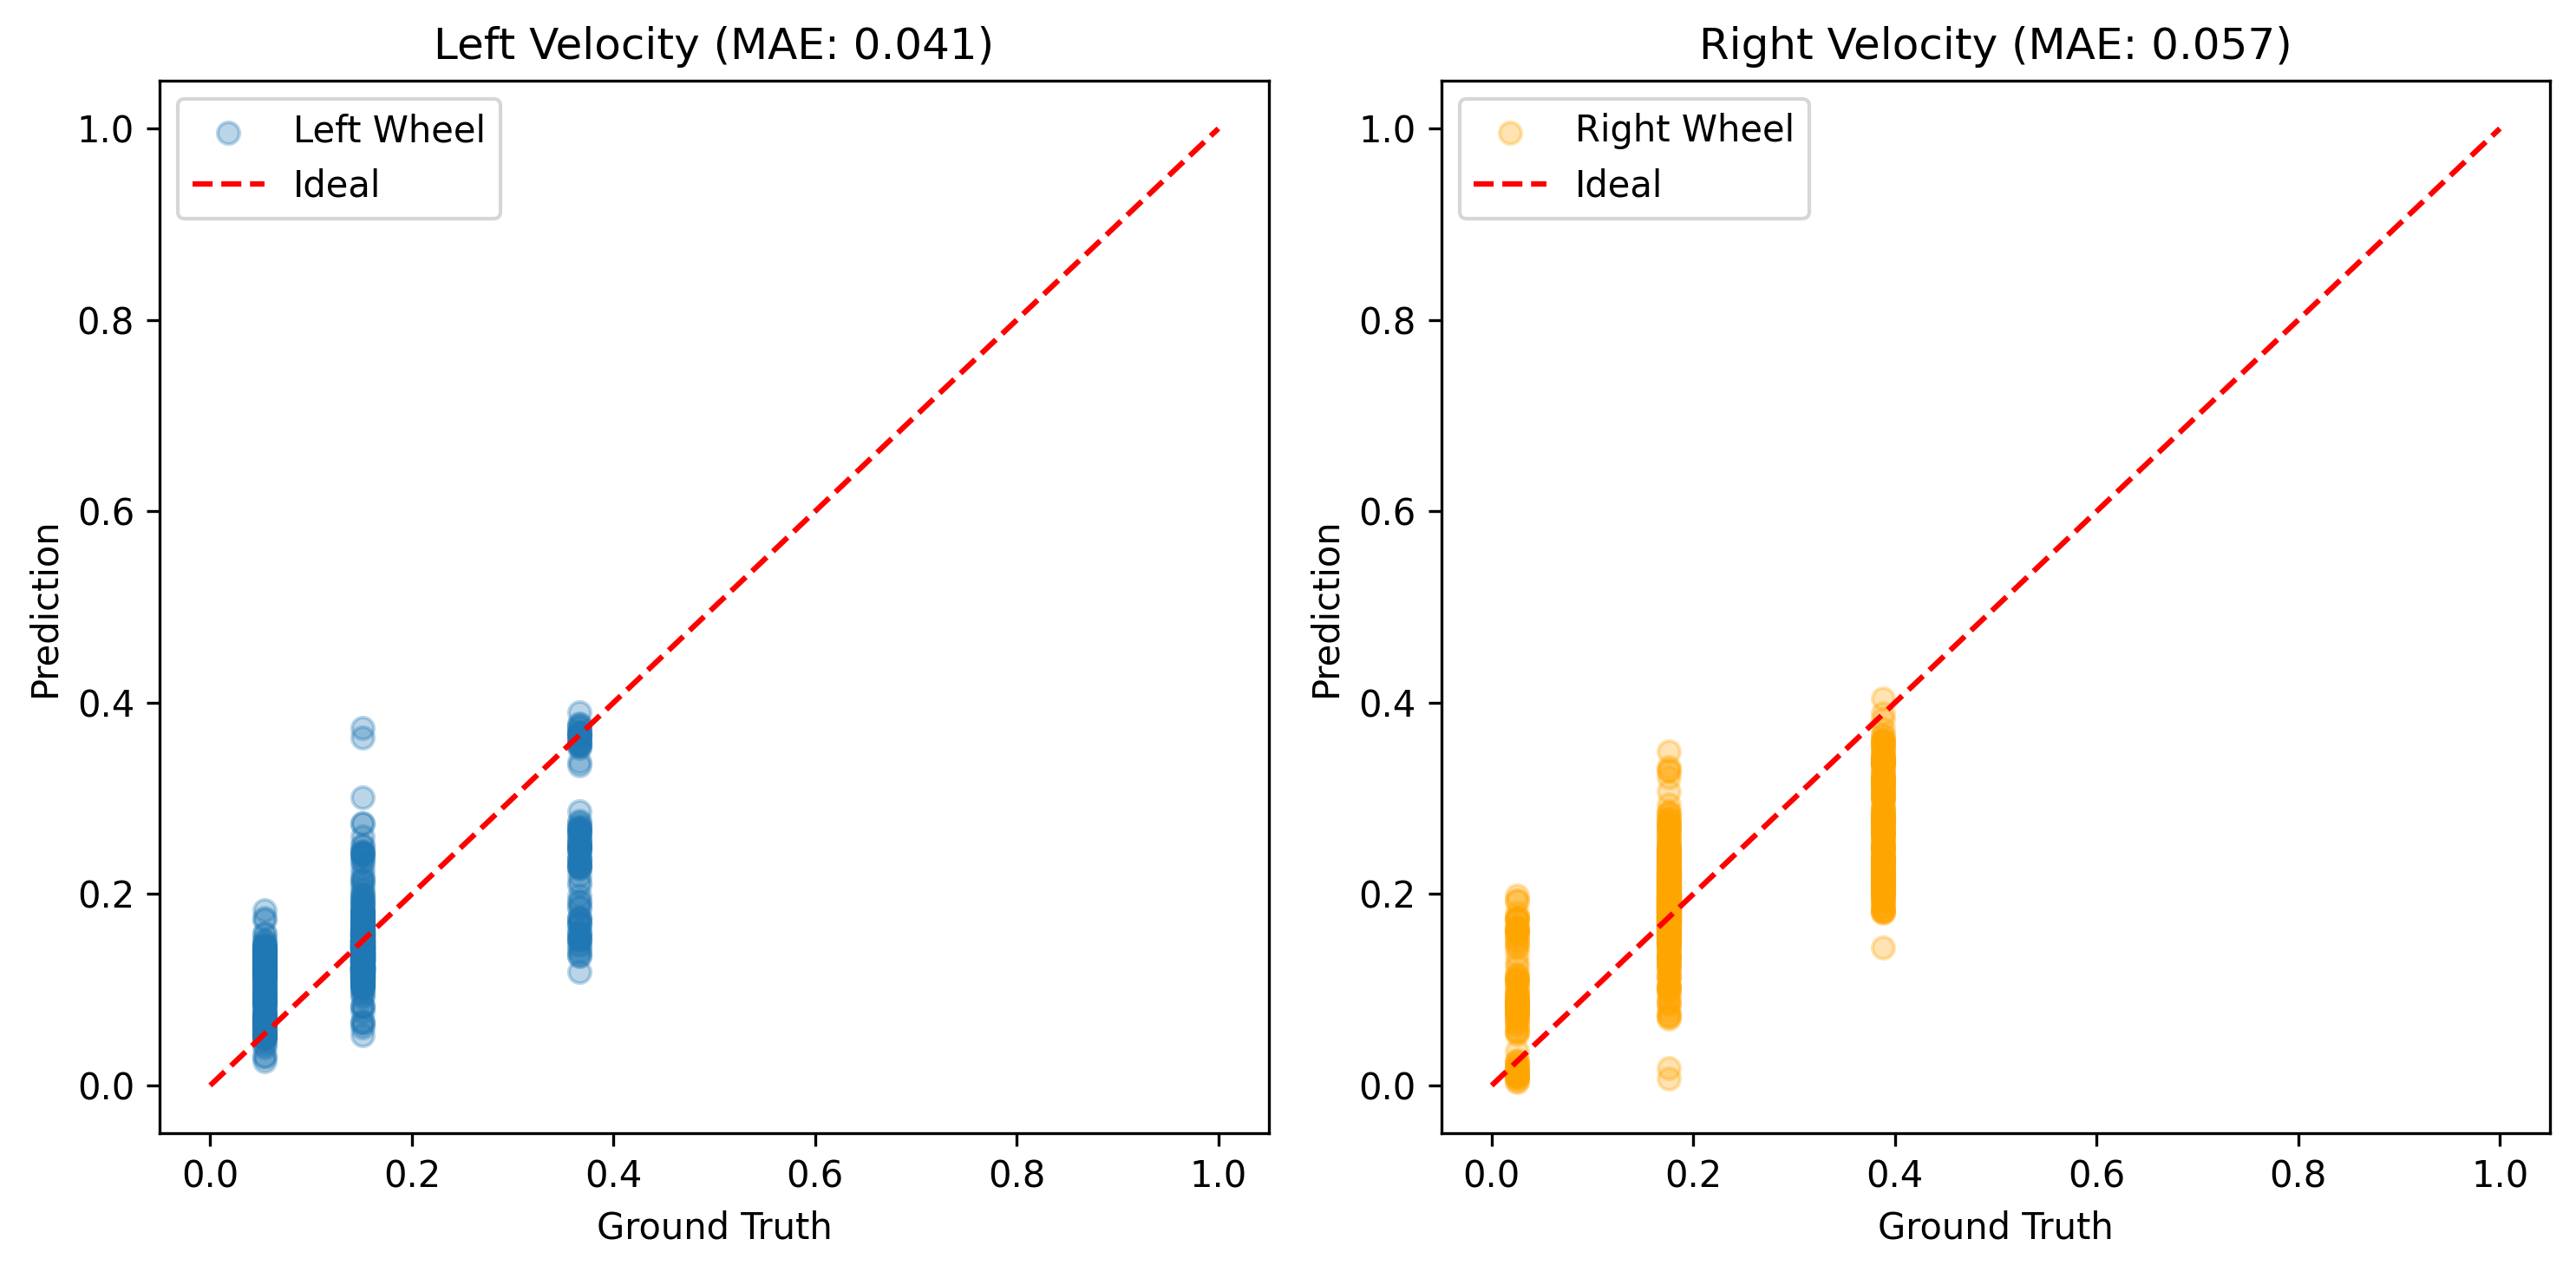
\includegraphics[width=\textwidth]{images/ablation/policy/irl_balanced_velocity_predictions.png}
        \caption{IRL2IRL}
    \end{subfigure}
    
    \begin{subfigure}[b]{0.8\textwidth}
        \centering
        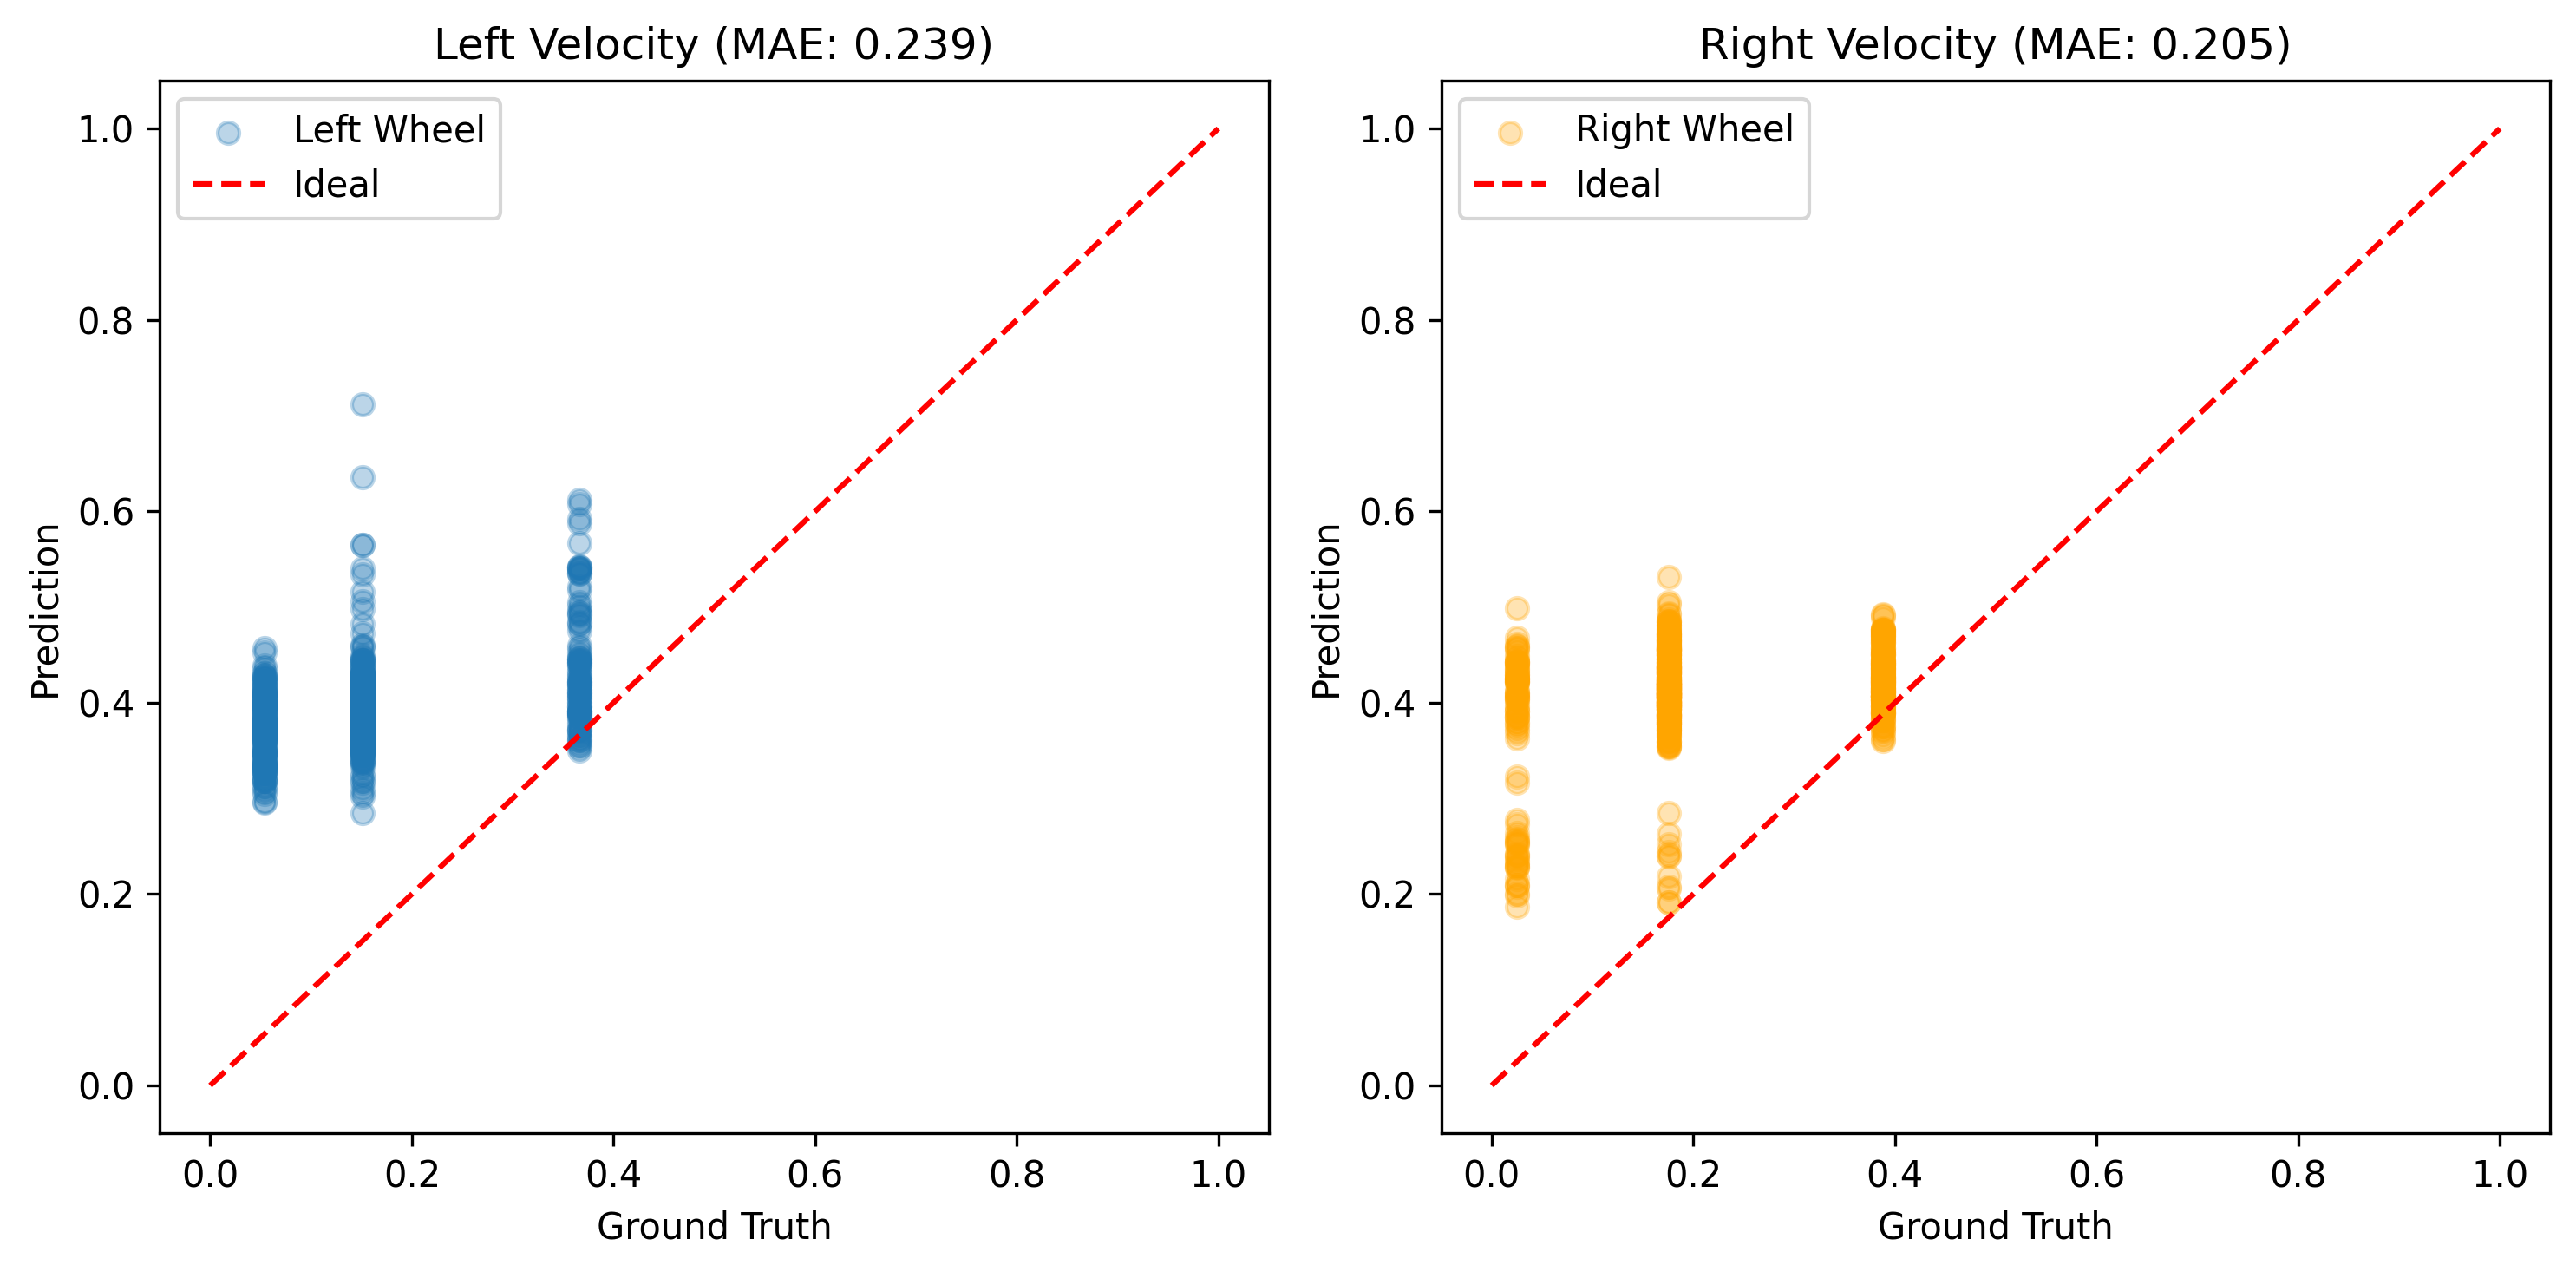
\includegraphics[width=\textwidth]{images/ablation/policy/sim_balanced_velocity_predictions_sim2irl.png}
        \caption{Sim2IRL}
    \end{subfigure}
    
    \begin{subfigure}[b]{0.8\textwidth}
        \centering
        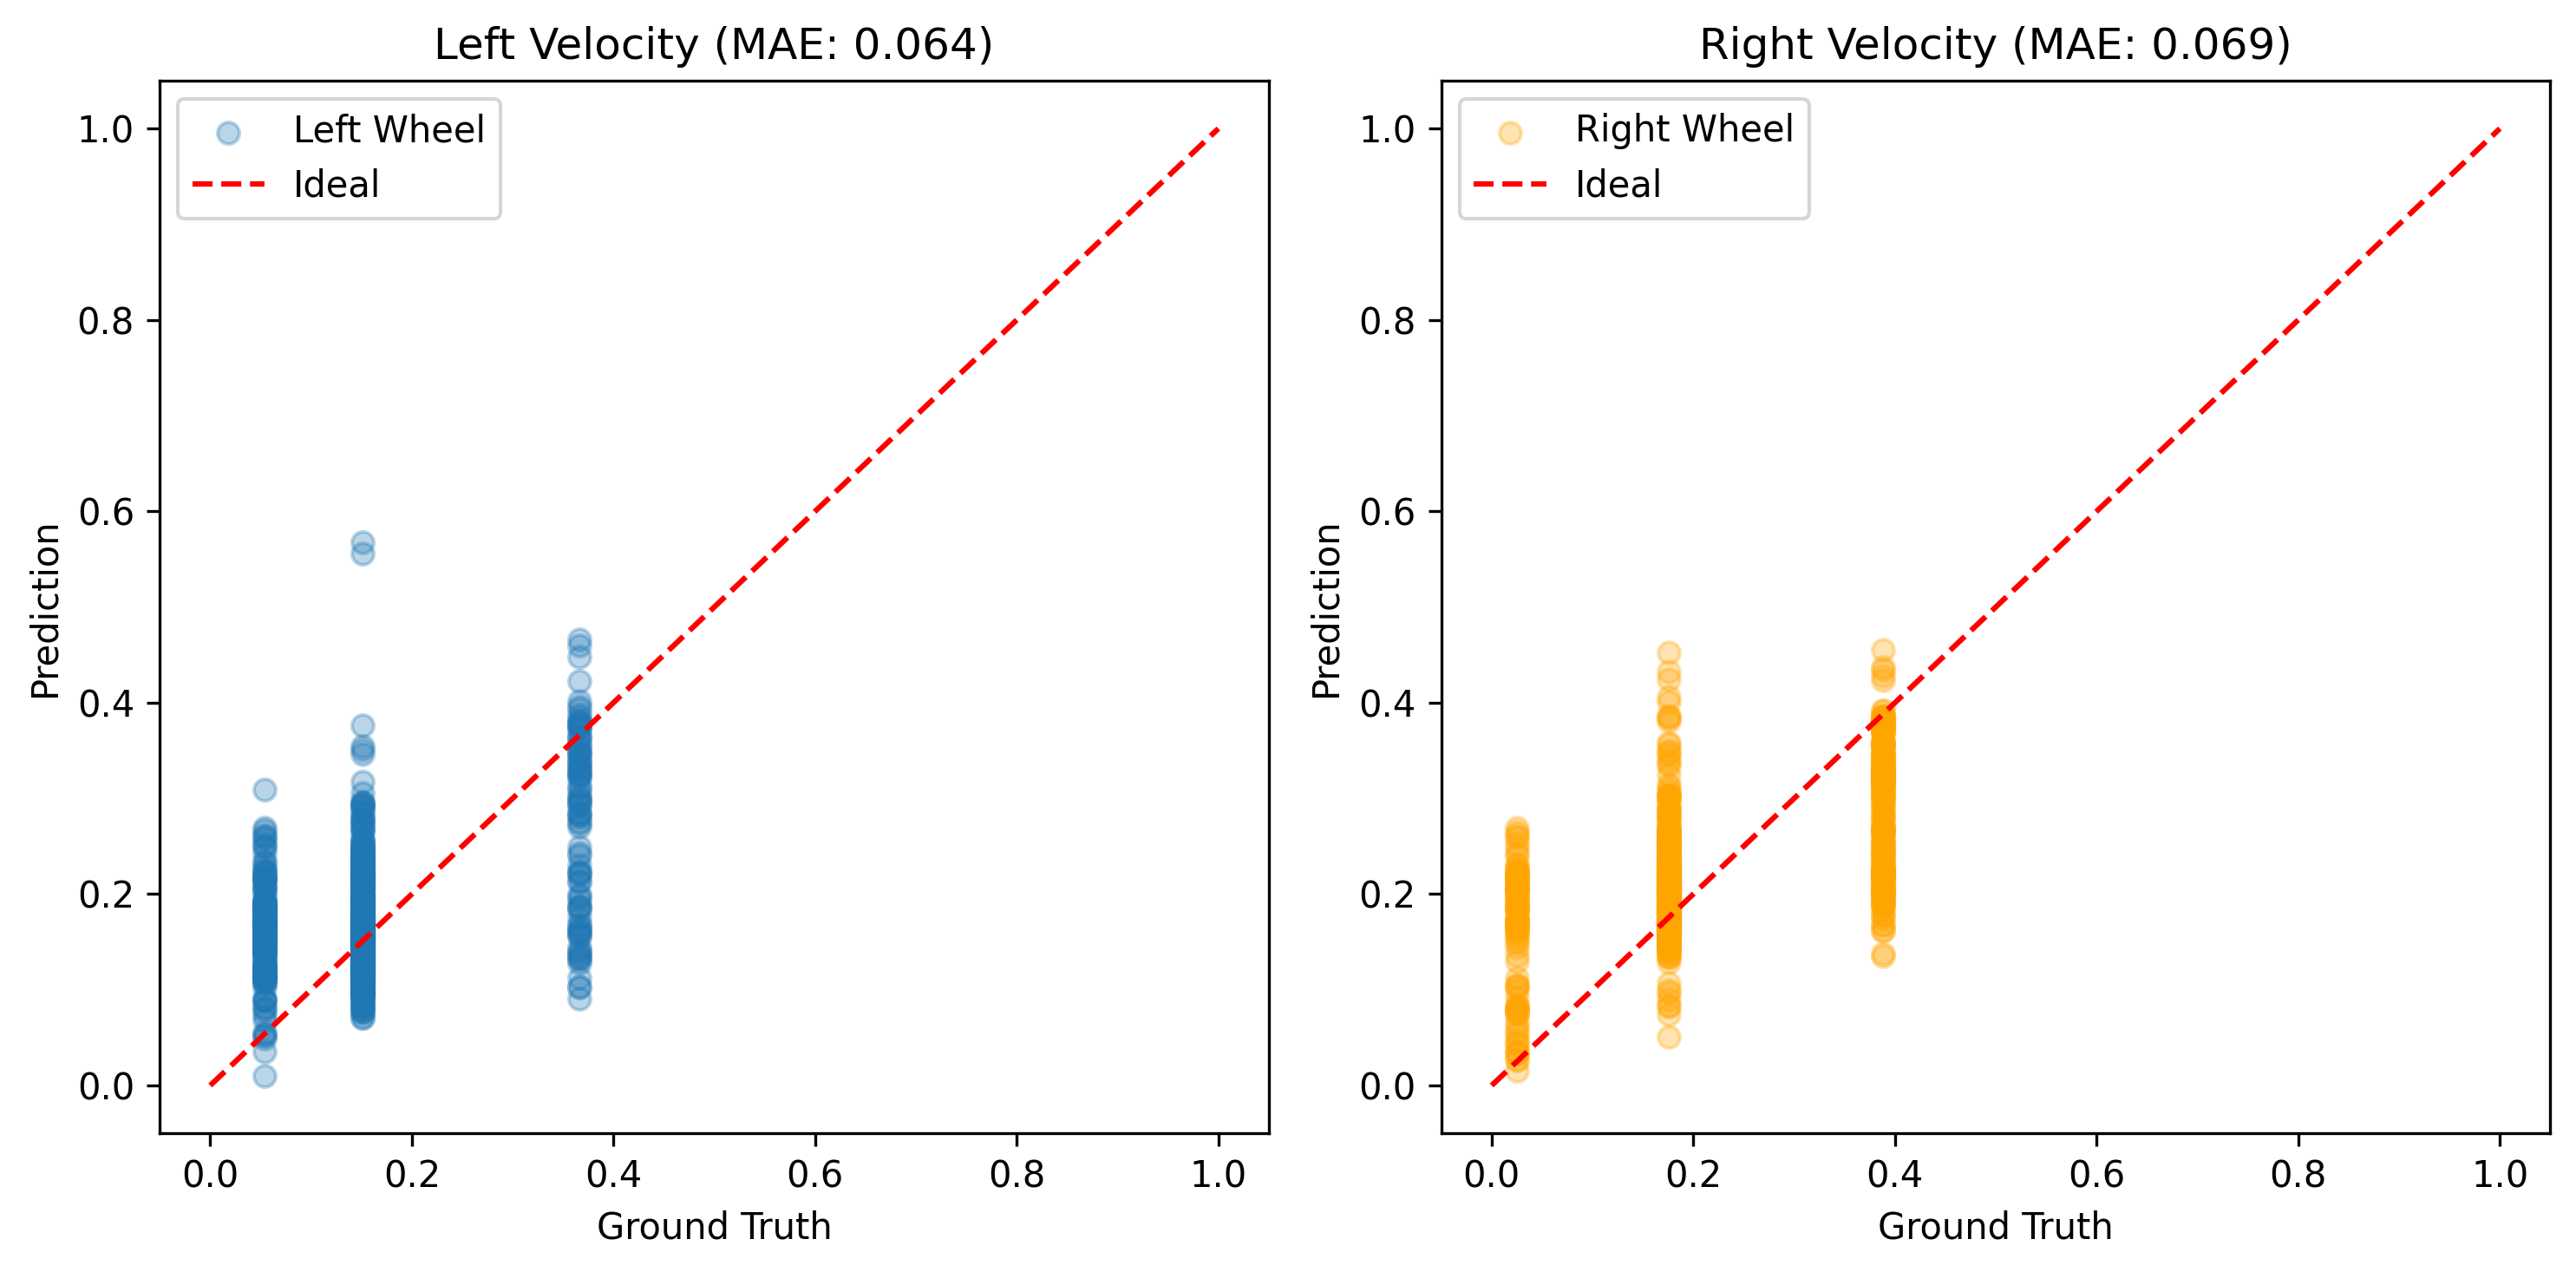
\includegraphics[width=\textwidth]{images/ablation/policy/mixed_balanced_velocity_predictions_mixed2irl.png}
        \caption{Mixed2IRL}
    \end{subfigure}
    \caption{\textbf{Performance Transfer:} Evaluation across different training policies.}
    \label{fig:perf_transfer}
\end{figure}
